\documentclass{article}

\usepackage[utf8]{inputenc}
\usepackage[spanish]{babel}

\usepackage[T1]{fontenc}

\usepackage{amsfonts}
\usepackage{amsmath}
\usepackage{amsthm}

\usepackage{verbatim}
\usepackage{newverbs}
\usepackage{graphicx}
\usepackage{xcolor}

\usepackage{geometry}

\spanishdecimal{.}

\DeclareMathOperator{\divop}{div}
\DeclareMathOperator{\rotop}{rot}
\def\Eqref#1{(\ref{#1})}

\setlength{\parskip}{\medskipamount}
\setlength{\parindent}{0pt}


\newcounter{maximaic}
\newcounter{maximaoc}

\setcounter{maximaic}{1}
\setcounter{maximaoc}{0}

\newenvironment{maximai}
{\noindent

 {\color{red}\bfseries (\% i\arabic{maximaic}) }
 \color{blue}\verb}{
\stepcounter{maximaic}
\stepcounter{maximaoc}

}
\newenvironment{maximal}
{\noindent
 \phantom{\color{red}\bfseries (\% i\arabic{maximaic}) }
 \color{blue}\verb}{

}

\newenvironment{maximao}
{
 {\bfseries\color{orange}(\% o\arabic{maximaoc}) }
 $ \displaystyle
  }{$

}

\newenvironment{maximaoo}
{
 \stepcounter{maximaic}
 \stepcounter{maximaoc}
 {\bfseries\color{orange}(\% o\arabic{maximaoc}) }
 $ \displaystyle
  }{$

}

% phantom version of maximaoo
\newenvironment{maximaop}
{
 \stepcounter{maximaic}
 \stepcounter{maximaoc}
 \phantom{{\bfseries\color{orange}(\% o\arabic{maximaoc}) }}
 $ \displaystyle
  }{$

}

\newenvironment{maximat}
{
 {\bfseries\color{orange}(\% t\arabic{maximaoc}) }
  }{

}

\newcommand{\maximain}[1]{\textcolor{blue}{\texttt{#1}}}


\def\enumalph{\renewcommand{\labelenumi}{$(\alph{enumi})$}}

\title{}
\author{}
\date{}

\begin{document}

\begin{minipage}{.4\textwidth}
	
\includegraphics[width=\linewidth]{uca.jpg}
\end{minipage}
%
\begin{minipage}{.6\textwidth}
	\begin{flushright}
		{\Large Matemáticas II}

		\medskip
		{\large Grado en química}

		\medskip
		Curso 2021-2022
	\end{flushright}
\end{minipage}

\medskip
\textbf{\Large Práctica 1. Introducción a la programación}

%%!TeX root=main.tex

\section{Listas y tablas}

\subsection*{Creando listas}

Las listas son objetos que almacenan valores de forma ordenada.
A continuación mostramos cómo se pueden crear listas a partir de
los valores que la forman.

\begin{maximai}
	lista:[2,-3,5,6];
\end{maximai}\begin{maximao}
	\left[ 2 , -3 , 5 , 6 \right]
\end{maximao}\begin{maximai}
	otralista:[1,2+1/2,[a,2,c],1+3*x+y^2];
\end{maximai}\begin{maximao}
	\left[ 1 , {{5}\over{2}} , \left[ a , 2 , c \right]  , y^2+3\,x+1
	\right]
\end{maximao}

Una lista puede no tener ningún valor, esta es la lista vacía.
\begin{maximai}
	listavacia:[];
\end{maximai}\begin{maximao}
	\left[\  \right]
\end{maximao}

Existe un tipo de lista especial, que llamamos tabla, este tipo de lista
almacena en cada entrada una nueva lista con la particularidad que todas
estas listas tienen el mismo número de elementos.

Por ejemplo una tabla almacenando dos valores cada vez.
\begin{maximai}
	tabla:[[1,2],[-3,4],[8,7],[-10,11]];
\end{maximai}\begin{maximao}
	\left[ \left[ 1 , 2 \right]  , \left[ -3 , 4 \right]  , \left[ 8 ,
	7 \right]  , \left[ -10 , 11 \right]  \right]
\end{maximao}
Y otro ejemplo de una tabla almacenando tres valores.
\begin{maximai}
	otratabla:[[1,2,2],[-3,8,4],[8,-2,7],[-10,99,11]];
\end{maximai}\begin{maximao}
	\left[ \left[ 1 , 2 , 2 \right]  , \left[ -3 , 8 , 4 \right]  ,
	\left[ 8 , -2 , 7 \right]  , \left[ -10 , 99 , 11 \right]  \right]
\end{maximao}

Anteriormente se han creado las listas expresando explícitamente todos
sus elementos, pero también hay posibilidades de crear listas a partir
de una expresión, esto se puede hacer con el comando
\maximain{create\_list}, su usa de la siguiente manera
\begin{center}
	\maximain{create\_list(expr, i, $\texttt{i}_0$, $\texttt{i}_1$)}
\end{center}
y crea la lista evaluando en expresión el valor de \maximain{i},
desde \maximain{$\texttt{i}_0$} hasta \maximain{$\texttt{i}_0$}.

\begin{maximai}
	create_list(2*i,i,1,10);
\end{maximai}\begin{maximao}
	\left[ 2 , 4 , 6 , 8 , 10 , 12 , 14 , 16 , 18 , 20 \right]
\end{maximao}

\begin{maximai}
	create_list([i, 2*i],i,1,10);
\end{maximai}\begin{maximao}
	\left[ \left[ 1 , 2 \right]  , \left[ 2 , 4 \right]  , \left[ 3 , 6
	\right]  , \left[ 4 , 8 \right]  , \left[ 5 , 10 \right]  , \left[
		6 , 12 \right]  , \left[ 7 , 14 \right]  , \left[ 8 , 16 \right]  ,
	\left[ 9 , 18 \right]  , \left[ 10 , 20 \right]  \right]
\end{maximao}

Otra manera de usar la función
\maximain{create\_list} es la siguiente
\begin{center}
	\maximain{create\_list(expr, i, lista)}
\end{center}
evaluando los valores de \maximain{i} en cada
valor de la lista \maximain{lista}.

\begin{maximai}
	xx:create_list(%pi*i/8, i, 1, 16);
\end{maximai}\begin{maximao}
	\left[ {{\pi}\over{8}} , {{\pi}\over{4}} , {{3\,\pi}\over{8}} , {{
		\pi}\over{2}} , {{5\,\pi}\over{8}} , {{3\,\pi}\over{4}} , {{7\,\pi
	}\over{8}} , \pi , {{9\,\pi}\over{8}} , {{5\,\pi}\over{4}} , {{11\,
	\pi}\over{8}} , {{3\,\pi}\over{2}} , {{13\,\pi}\over{8}} , {{7\,\pi
	}\over{4}} , {{15\,\pi}\over{8}} , 2\,\pi \right]
\end{maximao}\begin{maximai}
	puntos:create_list([x,sin(x)], x, xx);
\end{maximai}\begin{maximao}
	\left[ \left[ {{\pi}\over{8}} , \sin \left({{\pi}\over{8}}\right)
	\right]  , \left[ {{\pi}\over{4}} , {{1}\over{\sqrt{2}}} \right]
	, \left[ {{3\,\pi}\over{8}} , \sin \left({{3\,\pi}\over{8}}\right)
	\right]  ,
	%\left[ {{\pi}\over{2}} , 1 \right]  , \left[ {{5\,\pi
	%\over{8}} , \sin \left({{5\,\pi}\over{8}}\right) \right]  , \left[
	%{{3\,\pi}\over{4}} , {{1}\over{\sqrt{2}}} \right]  , \left[ {{7\,\pi
	%}\over{8}} , \sin \left({{7\,\pi}\over{8}}\right) \right]  , \left[
	%\pi , 0 \right]  , \left[ {{9\,\pi}\over{8}} , \sin \left({{9\,\pi
	%}\over{8}}\right) \right]  , \left[ {{5\,\pi}\over{4}} , -{{1}\over{
	%\sqrt{2}}} \right]  , \left[ {{11\,\pi}\over{8}} , \sin \left({{11\,
	%\pi}\over{8}}\right) \right]  , \left[ {{3\,\pi}\over{2}} , -1
	%\right]  , \left[ {{13\,\pi}\over{8}} , \sin \left({{13\,\pi}\over{
	%8}}\right) \right]  , \left[ {{7\,\pi}\over{4}} , -{{1}\over{\sqrt{2
	%}}} \right]
	\ldots
	, \left[ {{15\,\pi}\over{8}} , \sin \left({{15\,\pi
	}\over{8}}\right) \right]  , \left[ 2\,\pi , 0 \right]  \right]
\end{maximao}

Para obtener un elemento de una lista debemos indicar su posición
entre corchetes. Por ejemplo el primer elemento de \maximain{xx}.
\begin{maximai}
	xx[1];
\end{maximai}\begin{maximao}
	{{\pi}\over{8}}
\end{maximao}

O el elemento tercero de la tabla \maximain{puntos}.
\begin{maximai}
	puntos[3];
\end{maximai}\begin{maximao}
	\left[ {{3\,\pi}\over{8}} , \sin \left({{3\,\pi}\over{8}}\right)
	\right]
\end{maximao}

Este último a su vez es una lista, así que podríamos obtener
el segundo elemento del tercer elemento de la tabla \maximain{puntos}
de la siguiente manera.
\begin{maximai}
	puntos[3][2];
\end{maximai}\begin{maximao}
	\sin \left({{3\,\pi}\over{8}}\right)
\end{maximao}

El tamaño de una lista se puede obtener con la función
\maximain{length}.
\begin{maximai}
	length(xx);
\end{maximai}\begin{maximao}
	16
\end{maximao}\begin{maximai}
	length(puntos);
\end{maximai}\begin{maximao}
	16
\end{maximao}\begin{maximai}
	length(puntos[1]);
\end{maximai}\begin{maximao}
	2
\end{maximao}\begin{maximai}
	length([]);
\end{maximai}\begin{maximao}
	0
\end{maximao}

\subsection*{Representación de tablas}

Los puntos anteriores se podrían representar de la siguiente manera.

\begin{maximai}
	wxplot2d([discrete, puntos], [style,points]);
\end{maximai}\begin{maximat}
	\begin{center}
		\includegraphics[scale=.5]{wxplot2d_puntos.pdf}
	\end{center}
\end{maximat}

En el caso anterior se ha evaluado una función que ya
tiene definida maxima como \maximain{cos}.
Pero también se puede usar una función definida por el usuario.
\begin{maximai}
	f(x):=x^3-3*x^2+5*x-2$
\end{maximai}\begin{maximai}
	xx2:create_list(2*i+1, i, 0, 4);
\end{maximai}\begin{maximao}
	\left[ 1 , 3 , 5 , 7 , 9 \right]
\end{maximao}\begin{maximai}
	puntos2:create_list(f(x),x,xx2);
\end{maximai}\begin{maximao}
	\left[ 1 , 13 , 73 , 229 , 529 \right] 
\end{maximao}\begin{maximai}
	wxplot2d([discrete, puntos2], [style,points]);
\end{maximai}\begin{maximat}
	\begin{center}
		\includegraphics[scale=.5]{wxplot2d_puntos2.pdf}
	\end{center}
\end{maximat}

En el ejemplo anterior se ha representado los puntos
de la función $f$ en los que los valores
de abscisas son los números impares del 1 al 9.


\subsection*{Operaciones sobre listas}

A partir de listas se pueden calcular nuevas listas.
Una posibilidad es aplicar operaciones artiméticas
entre listas.

\begin{maximai}
	a:[1,2,3,4,5]$
\end{maximai}\begin{maximal}
	b:[6,7,8,9,0]$
\end{maximal}
\begin{maximai}
	a+b;
\end{maximai}\begin{maximao}
	\left[ 7 , 9 , 11 , 13 , 5 \right]
\end{maximao}\begin{maximai}
	a-b;
\end{maximai}\begin{maximao}
	\left[ -5 , -5 , -5 , -5 , 5 \right]
\end{maximao}\begin{maximai}
	a*b;
\end{maximai}\begin{maximao}
	\left[ 6 , 14 , 24 , 36 , 0 \right]
\end{maximao}\begin{maximai}
	b/a;
\end{maximai}\begin{maximao}
	\left[ 6 , {{7}\over{2}} , {{8}\over{3}} , {{9}\over{4}} , 0
	\right]
\end{maximao}\begin{maximai}
	a^2;
\end{maximai}\begin{maximao}
	\left[ 1 , 4 , 9 , 16 , 25 \right]
\end{maximao}\begin{maximai}
	sqrt(b);
\end{maximai}\begin{maximao}
	\left[ \sqrt{6} , \sqrt{7} , 2^{{{3}\over{2}}} , 3 , 0 \right]
\end{maximao}

Como vemos las operaciones se aplica elemento a elemento.

El producto escalar se calcula con el operador punto (\maximain{.}).
\begin{maximai}
	a.b;
\end{maximai}\begin{maximao}
	80
\end{maximao}

Existen otras operaciones definidas en maxima como las que veremos
a continuación, pero para ello definamos previamente una lista para
y una tabla.

\begin{maximai}
	lista1:[2,-3,5,6];
\end{maximai}\begin{maximao}
	\left[ 2 , -3 , 5 , 6 \right]
\end{maximao}\begin{maximai}
	tabla:[[1,2],[-3,4],[8,7],[-10,11]];
\end{maximai}\begin{maximao}
	\left[ \left[ 1 , 2 \right]  , \left[ -3 , 4 \right]  , \left[ 8 ,
	7 \right]  , \left[ -10 , 11 \right]  \right]
\end{maximao}

\begin{itemize}

	\item \maximain{delete}. Devuelve una nueva lista con los valores
		eliminados.
		\begin{maximai}
			lista2:delete(-3,lista1);
		\end{maximai}\begin{maximao}
			\left[ 2 , 5 , 6 \right]
		\end{maximao}

	\item \maximain{cons}. Devuelve una nueva lista añadiendo al principio
		de la lista el valor que se indique.
		\begin{maximai}
			lista3:cons(-5,lista1);
		\end{maximai}\begin{maximao}
			\left[ -5 , 2 , -3 , 5 , 6 \right]
		\end{maximao}

	\item \maximain{append}. Calcula una nueva lista uniendo la primera
		lista con la segunda.
		\begin{maximai}
			lista4:append(lista2,lista3);
		\end{maximai}\begin{maximao}
			\left[ 2 , 5 , 6 , -5 , 2 , -3 , 5 , 6 \right]
		\end{maximao}

	\item \maximain{reverse}. Calcula una nueva lista cambiando los
		valores de orden.
		\begin{maximai}
			lista5:reverse(lista4);
		\end{maximai}\begin{maximao}
			\left[ 6 , 5 , -3 , 2 , -5 , 6 , 5 , 2 \right]
		\end{maximao}

	\item \maximain{unique}. Devuelve una nueva lista eliminando los
		valores repetidos.
		\begin{maximai}
			lista6:unique(lista5);
		\end{maximai}\begin{maximao}
			\left[ -5 , -3 , 2 , 5 , 6 \right]
		\end{maximao}

	\item \maximain{sort}. Calcula una nueva lista ordenando los valores
		de menor a mayor.
		\begin{maximai}
			lista7:sort(lista6);
		\end{maximai}\begin{maximao}
			\left[ -5 , -3 , 2 , 5 , 6 \right]
		\end{maximao}

	\item \maximain{flatten}. Esta función aplicada a una tabla unifica
		los valores en una única lista.
		\begin{maximai}
			flatten(tabla);
		\end{maximai}\begin{maximao}
			\left[ 1 , 2 , -3 , 4 , 8 , 7 , -10 , 11 \right]
		\end{maximao}

\end{itemize}

\subsection*{Ejercicios}

\begin{enumerate}

	\item \begin{enumerate}
			\item Definir la función $f(k)=\frac{2k\pi}{6}$.
			\item Definir una lista evaluando la función en los valores
				$k=0,\ldots,5$.
			\item Crear una lista de puntos $(\cos x, \sin x)$, para
				cada valor de $x$ de la lista anterior.
			\item Representar gráficamente los puntos anteriores.
	\end{enumerate}

\item \begin{enumerate}
		\item Definir la función
			\begin{equation*}
				f(x) = \left( \frac{\sqrt{2}\cos x}{\sin^2 x +1},
				\frac{\sqrt{2}\cos x\sin x}{\sin^2 x +1},\right).
			\end{equation*}
		\item Crear una lista de valores desde 0 hasta 10,
			con un espacio entre valores de $0.1$
		\item Crear una tabla con las imágenes de $f$ en los
			valores anteriores.
		\item Representar gráficamente la tabla anterior.
\end{enumerate}

		\item \begin{enumerate}
				\item Crear una tabla de 5 elementos con los puntos
					$(n,2n^3,n-2)$ empezando en $n=0$.
				\item Obtener el elemento cuarto de la tabla anterior.
				\item Obtener el elemento segundo del tercer elemento
					de la tabla.
				\item Escribir la tabla como una única lista.
				\item Ordenar la lista anterior.
				\item Ordenar la lista de mayor a menor.
		\end{enumerate}

\end{enumerate}

%%!TeX root=main.tex

\section{Funciones}

Maxima ya incorpora algunas funciones ya definidas,
pero también se pueden incorporar funciones definidas
por el usuario.
Cuando nos referimos a funciones en maxima no solamente
nos referimos a las funciones matemáticas con valores numéricos,
sino a funciones que pueden usar todo tipo de datos de maxima.
Un ejemplo de funciones que no son matemáticas son las funciones
que se aplican a las listas.

Las funciones sirven para automatizar un proceso con datos sin determinar,
estos son los argumentos, que a la hora de usar la función toman los valores
que se le indique.

Por ejemplo, podríamos definir el logaritmo en base 2 como mostramos.
\begin{maximai}
	log2(x):=log(x)/log(2)$
\end{maximai}

Y usar la función de la siguiente forma.
\begin{maximai}
	log2(32),numer;
\end{maximai}\begin{maximao}
	5.0
\end{maximao}

Y también se podría definir el logaritmo en base 3, 4, 5, \ldots
pero entonces nos damos cuenta que la base también puede ser un argumento
de la función, y así tendríamos todas las posibilidades.

\begin{maximai}
	logb(x,b):=log(x)/log(b)$
\end{maximai}\begin{maximai}
	logb(25,5),numer;
\end{maximai}\begin{maximao}
	2.0
\end{maximao}

A veces hace falta definir funciones que hacen algunos cálculos
intermedios, en este caso hay que definir la función con un comando
conocido como \maximain{block}.


\begin{maximai}
	f1(a,b,c):=block([u,v], u:b-c, v:a-b, u/v)$
\end{maximai}
\begin{maximai}
	f1(2,3,1);
\end{maximai}\begin{maximao}
	-2
\end{maximao}

En el ejemplo anterior se han usado las variables \maximain{u} y
\maximain{v} para guardar los cálculos intermedios, y el resultado
que se calcula en la función es el último, \maximain{u/v}.

\begin{maximai}
	f2(y):=block([u:y^2], u:u+3, u:u^2, u)$
\end{maximai}
\begin{maximai}
	f2(4);
\end{maximai}\begin{maximao}
	361
\end{maximao}

En el ejemplo anterior la variable auxiliar \maximain{u} se inicializa
con una expresión del argumento.

En ciertas ocasiones es útil escribir un mensaje por pantalla en cierto
momento en el cálulo de la función.


\begin{maximai}
	f3(x):=block(print("saludos"),x^2+1)$
\end{maximai}\begin{maximai}
	f3(-1);
\end{maximai}\begin{maximaop}
	\text{saludos}
\end{maximaop}\begin{maximao}
	2
\end{maximao}

En el siguiente ejemplo mostramos como se repite la llamada de la función.

\begin{maximai}
	create_list(f3(i^2),i,1,3);
\end{maximai}\begin{maximaop}
	\text{saludos}
\end{maximaop}\begin{maximaop}
	\text{saludos}
\end{maximaop}\begin{maximaop}
	\text{saludos}
\end{maximaop}\begin{maximao}
	\left[ 2 , 17 , 82 \right]
\end{maximao}

A continuación se muestra cómo se crearía una función que calcula
el módulo de un número imaginario.

\begin{maximai}
	f4(x,y):=block([re,im,g:x+%i*y], re:realpart(g), im:imagpart(g),
\end{maximai}\begin{maximal}
	sqrt(re^2+im^2))$
\end{maximal}\begin{maximai}
	f4(2,-1);
\end{maximai}\begin{maximao}
	\sqrt{5}
\end{maximao}

Existe una forma para admitir un número indeterminado de argumentos.

\begin{maximai}
	sumdif([x]):=x^2 . create_list( (-1)^(k+1),k,1,length(x))$
\end{maximai}\begin{maximai}
	sumdif(a,b,c,d,e,f,g);
\end{maximai}\begin{maximao}
	g^2-f^2+e^2-d^2+c^2-b^2+a^2
\end{maximao}\begin{maximai}
	sumdif(1,1,-1,0,4,5,0,-8,9,-1);
\end{maximai}\begin{maximao}
	8
\end{maximao}\begin{maximai}
	sumdif(2,u+v);
\end{maximai}\begin{maximao}
	4-\left(v+u\right)^2
\end{maximao}

Una función se puede pasar como argumento al definir una función.

\begin{maximai}
	funfun(G,a):=G(a^2)^2;
\end{maximai}\begin{maximai}
	funfun(log,2);
\end{maximai}\begin{maximao}
	\left(\log 4\right)^2
\end{maximao}

\begin{maximai}
	funfun2(G,[x]):=G(x)$
\end{maximai}\begin{maximai}
	funfun2(sin,%pi,%pi/2);
\end{maximai}\begin{maximao}
	\left[ 0 , 1 \right]
\end{maximao}

Un argumento de la función puede también ser una lista,
a continuación mostramos un ejemplo de ello.

\begin{maximai}
	ultimodelalista(L):=L[length(L)];
\end{maximai}\begin{maximai}
	ultimodelalista([1,-1,3,22,35,7]);
\end{maximai}\begin{maximao}
	7
\end{maximao}

\subsection*{Ejercicios}

\begin{enumerate}
		
	\item % raíz n-ésima
		Cree una función \maximain{raizn($a$,$n$)} que calcule la raíz
		\maximain{$n$}-ésima del número \maximain{$a$}.

	\item % derivada n-ésima de la función seno en un punto x
		Cree una función \maximain{dsen($x$,$n$)} que calcule la derivada
		\maximain{$n$}-ésima de la función $\sin$ en el punto \maximain{$x$}.


	\item % crear una función mayoramenor que calcule una lista
		% de mayor a menor... argumento...
		Cree una función que tenga como argumento una lista y
		calcule la lista ordenada de mayor a menor.

	\item % el ejercicio 1 de la práctica de listas creaba
		% una lista de puntos que formaban un hexágono,
		% generalizar ...
		% creando una función que admita, n, como argumento
		% y genere una lista con los puntos formando un
		% polígono regular de n puntos.
		% el nombre de la función será poligonoregular(n)
		% probarlo con el siguiente comando
		% wxplot2d([discrete, poligonoregular(n)], [style,points]);
		En el ejercicio 1 de la práctica sobre listas se calculaba
		una lista de puntos que eran los vértices de un hexágono regular.
		En este ejercicio se pide generalizarlo creando una función
		\maximain{poligonoregular($n$)} que devuelva una lista de puntos
		que sean los vértices de un polígono regular de \maximain{$n$} vértices.
		Compruebese la solución graficando los puntos.

	%\item % la función max(a,b,...) devuelve el máximo de los
		% valores. Pero no funciona con listas es decir
		% max([3,2]) no devuelve el máximo de la lista
		% crear la función maxlist(l) que admite una lista
		%La función \maximain{max($a$,$b$,\ldots)} está definida por maxima

\end{enumerate}

%!TeX root=main.tex

\section{Lógica}

\subsection*{Valores lógicos}

En lógica se estudia la veracidad de las proposiciones,
esto es, si una proposición puede ser cierta o falsa.
En maxima existe los valores
\maximain{true} y \maximain{false}.
Aunque cuando se hace comprobaciones de variables que
no conoce ni sus valores ni ninguna propiedad puede que
resulte en \maximain{unknown}.
A continuación mostramos algunos ejemplos.

\begin{maximai}
is(2<3);
\end{maximai}
\begin{maximao}
\mathbf{true}
\end{maximao}

\begin{maximai}
is(3<2);
\end{maximai}
\begin{maximao}
\mathbf{false}
\end{maximao}

\begin{maximai}
is(a<b);
\end{maximai}
\begin{maximao}
{\it unknown}
\end{maximao}

El comando \maximain{is} da la información sobre la veracidad
de una expresión.

\subsection*{Operaciones de comparación}

Existen relaciones entre números,
por ejemplo igualdad, mayor igual, menor, \ldots,
estas relaciones pueden ser ciertas o falsas.
En maxima existen relaciones de comparación, a continuación
se muestran.
\begin{itemize}
	\item \maximain{=}. Igualdad.
	\item \maximain{\#}. Distinto.
	\item \maximain{<}. Menor.
	\item \maximain{<=}. Menor o igual.
	\item \maximain{>}. Mayor.
	\item \maximain{>=}. Mayor o igual.
\end{itemize}

Estas relaciones se pueden usar dentro del comando
\maximain{is}, como se ha visto en la sección anterior.

\subsection*{Operadores lógicos}

Existen operaciones entre los valores lógicos,
estos son operadores lógicos.
Algunos operadores lógicos se muestran a continuación.
\begin{itemize}
	\item \maximain{and}. Este operador es el ``y'' lógico.
		Devuelve \maximain{true} siempre que todos los operandos
		son ciertos, en otro caso es \maximain{false}.
	\item \maximain{or}. Este operador es el ``o'' lógico.
		Devuelve \maximain{true} siempre que exista al menos
		un operando que sea cierto, en otro caso es \maximain{false}.
	\item \maximain{not}. Este es el operador negación, y solamente
		acepta un operando, devolviendo el valor opuesto.
\end{itemize}

Las operaciones anteriores sirven para comprobar diferentes situaciones.
Por ejemplo para probar que la variable \maximain{a} está en el intervalo
$[0,1]$ se puede hacer lo siguiente.

\begin{maximai}
is(0<a and a<1);
\end{maximai}
\begin{maximao}
{\it unknown}
\end{maximao}

El caso anterior el resultado es \textit{unknown} ya que la variable
\maximain{a} no tiene ningún valor.

Además de valores numéricos se pueden comparar expresiones,
recuerde que en maxima se trabaja por defecto con expresiones simbólicas.
Dos expresiones pueden resultar falsas comprobadas de forma simbólicas
aunque algebraicamente sean iguales, esto se debe a que la igualdad
de expresiones en maxima se verifica cuando está escrita de la misma manera.
Obsevese el siguiente ejemplo.

\begin{maximai}
is((x+1)^2=x^2+2*x+1);
\end{maximai}
\begin{maximao}
\mathbf{false}
\end{maximao}

\begin{maximai}
is(expand((x+1)^2)=x^2+2*x+1);
\end{maximai}
\begin{maximao}
\mathbf{true}
\end{maximao}

\subsection*{Suposiciones}

En ciertas ocasiones es necesario suponer que
una variable verifica alguna condición.
Los comandos \maximain{assume} y \maximain{forget}
sirven para ello.
Veamos cómo funciona en el siguiente caso.
Por una parte sabemos lo siguiente.

\begin{maximai}
is((x+1)^2>=0);
\end{maximai}
\begin{maximao}
\mathbf{true}
\end{maximao}

Pero si $x\neq-1$ entonces debería ser cierto que
\maximain{(x+1)\^{}2>0}.
Para que maxima tenga en cuenta que la variable \maximain{x}
verifica que es distinto a $-1$ y comprobar la desigualdad
anterior se procede como sigue.

\begin{maximai}
assume(notequal(x,-1));
\end{maximai}
\begin{maximao}
\left[ {\it notequal}\left(x , -1\right) \right] 
\end{maximao}

\begin{maximai}
is((x+1)^2>0);
\end{maximai}
\begin{maximao}
\mathbf{true}
\end{maximao}

A partir de ahora maxima ya sabe que $\maximain{x}\neq-1$.
Para que deje de suponer la condición anterior habrá que usar
\maximain{forget}.

\begin{maximai}
forget(notequal(x,-1));
\end{maximai}
\begin{maximao}
\left[ {\it notequal}\left(x , -1\right) \right] 
\end{maximao}

A partir de ahora se tiene lo siguiente.

\begin{maximai}
is((x+1)^2>0);
\end{maximai}
\begin{maximao}
{\it unknown}
\end{maximao}

%!TeX root=main.tex

\section{Condicionales}

%\subsection*{Uso de \maximain{if}}
La orden condicional \maximain{if} es una sentencia
que comprueba si se verifica una condición,
si es verdadera ejecutará la expresión a continuación
del \maximain{then} y si es falsa ejecutará la
expresión después de \maximain{else}. La última es
opcional.

\begin{center}
	\maximain{if} condición \maximain{then} expr1
\end{center}
\begin{center}
	\maximain{if} condición \maximain{then} expr1
	\maximain{else} expr2
\end{center}

\begin{maximai}
if sin(4) < 9/10 and 2^2=4 then 1 else -1;
\end{maximai}
\begin{maximao}
1
\end{maximao}

\begin{maximai}
if sin(4) < -9/10 or 2^2=5 then 1 else -1;
\end{maximai}
\begin{maximao}
-1
\end{maximao}

\begin{maximai}
if sin(4)>cos(5) then 1;
\end{maximai}
\begin{maximao}
\mathbf{false}
\end{maximao}

\begin{maximai}
if sin(4)<cos(5) then 1;
\end{maximai}
\begin{maximao}
1
\end{maximao}

La sentencia condicional \maximain{if} es necesaria para definir
funciones a trozos. Por ejemplo para definir la función
\begin{equation*}
	F(x)=\left\{ \begin{array}{cl}
		0 & \text{ si } x<0, \\
		x^2 & \text{ si } x\geq0. \\
	\end{array}\right.
\end{equation*}

\begin{maximai}
F(x):=if x<0 then 0 else x^2$
\end{maximai}

\begin{maximai}
F(-1); F(0); F(3);
\end{maximai}
\begin{maximao}
0
\end{maximao}
\begin{maximaoo}
0
\end{maximaoo}
\begin{maximaoo}
9
\end{maximaoo}

%c F(x):=if x<0 then 0 else x^2$
%c plot2d(F(x),[x,-1,1],[y,-1,1], [pdf_file, "./plot_F.pdf"])$
%x
\begin{maximai}
	wxplot2d(F(x),[x,-1,1],[y,-1,1])$
\end{maximai}\begin{maximat}
	\begin{center}
		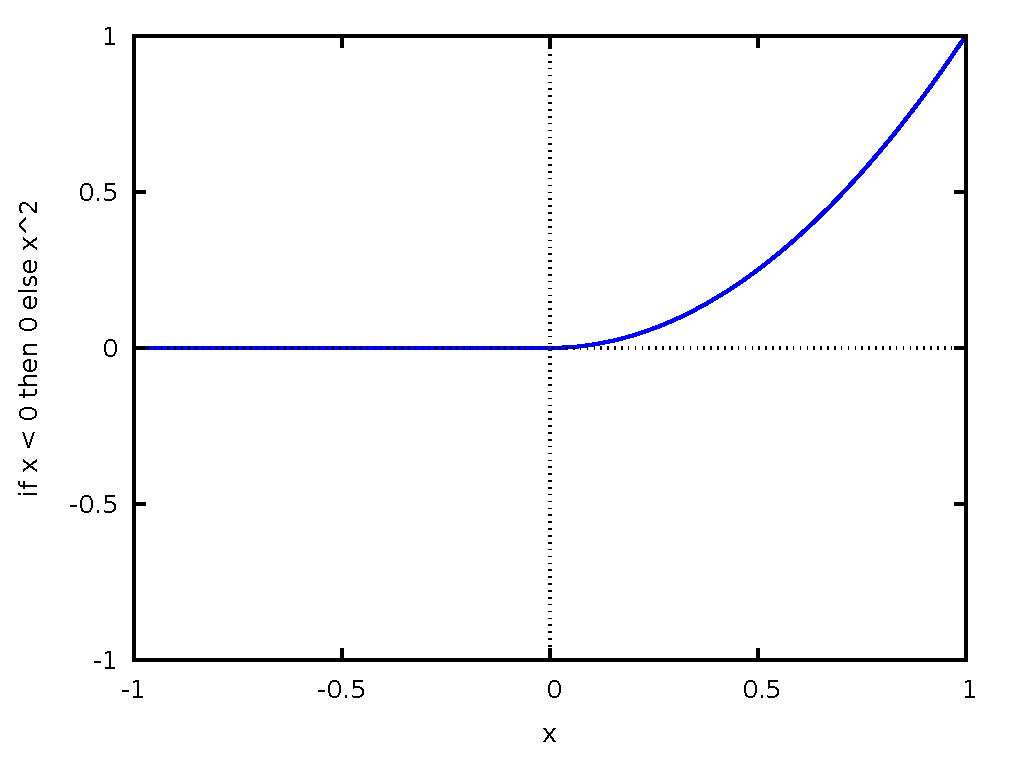
\includegraphics[scale=.5]{plot_F.pdf}
	\end{center}
\end{maximat}

A continaución definamos una función que está definida por
partes en tres intervalos diferentes.
\begin{equation*}
	G(x)=\left\{ \begin{array}{cl}
		0 & \text{ si } x<0, \\
		1 & \text{ si } 0\leq x\leq 1, \\
		x^2 & \text{ si } x>1. \\
	\end{array}\right.
\end{equation*}

\begin{maximai}
G(x):=if x<0 then 0 else (if x>1 then x^2 else 1)$
\end{maximai}

\begin{maximai}
G(.5);
\end{maximai}
\begin{maximao}
1
\end{maximao}

%c G(x):=if x<0 then 0 else (if x>1 then x^2 else 1)$
%c plot2d(G(x),[x,-1,3],[y,-1,9], [pdf_file, "./plot_G.pdf"])$
%x
\begin{maximai}
	wxplot2d(G(x),[x,-1,3],[y,-1,9])$
\end{maximai}\begin{maximat}
	\begin{center}
		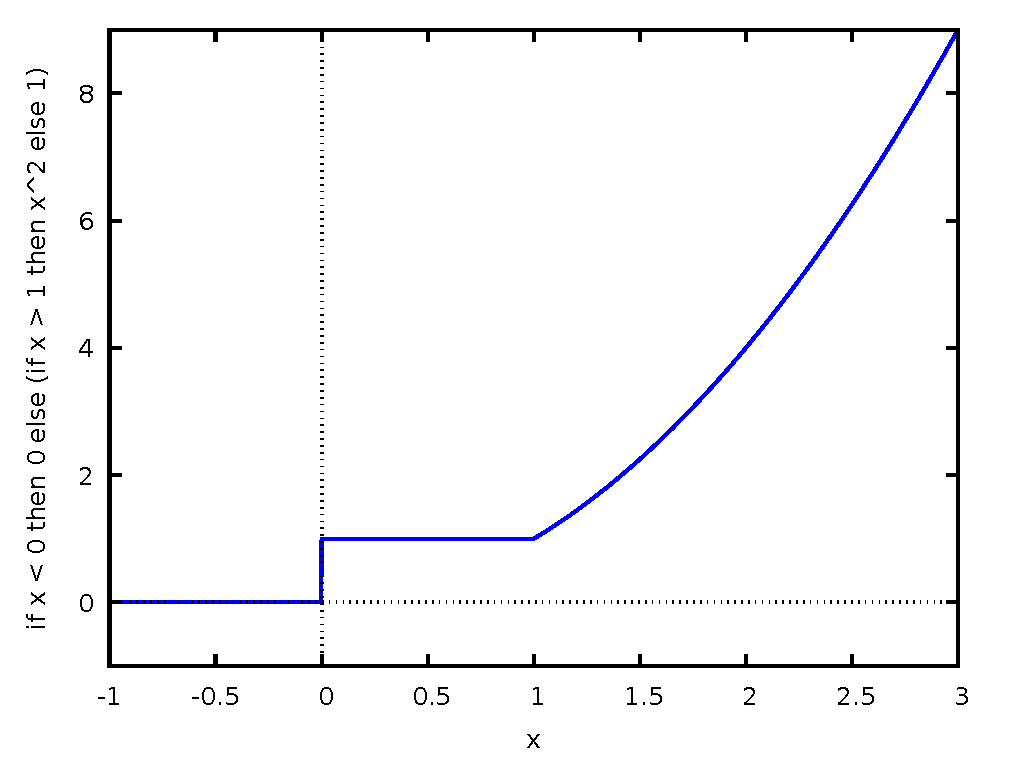
\includegraphics[scale=.5]{plot_G.pdf}
	\end{center}
\end{maximat}

En el caso anterior se dice que los \maximain{if} están anidados.
Ya que este uso es muy frecuente en programación, maxima incorpora
una palabra especial llamada \maximain{elseif}.
De este modo la función anterior se podría definir más facilmente.

\begin{maximai}
G(x):=if x<0 then 0 elseif x>1 then x^2 else 1$
\end{maximai}

%c G(x):=if x<0 then 0 elseif x>1 then x^2 else 1$
%c plot2d(G(x),[x,-1,3],[y,-1,9], [pdf_file, "./plot_G2.pdf"])$
%x
\begin{maximai}
	wxplot2d(G(x),[x,-1,3],[y,-1,9])$
\end{maximai}\begin{maximat}
	\begin{center}
		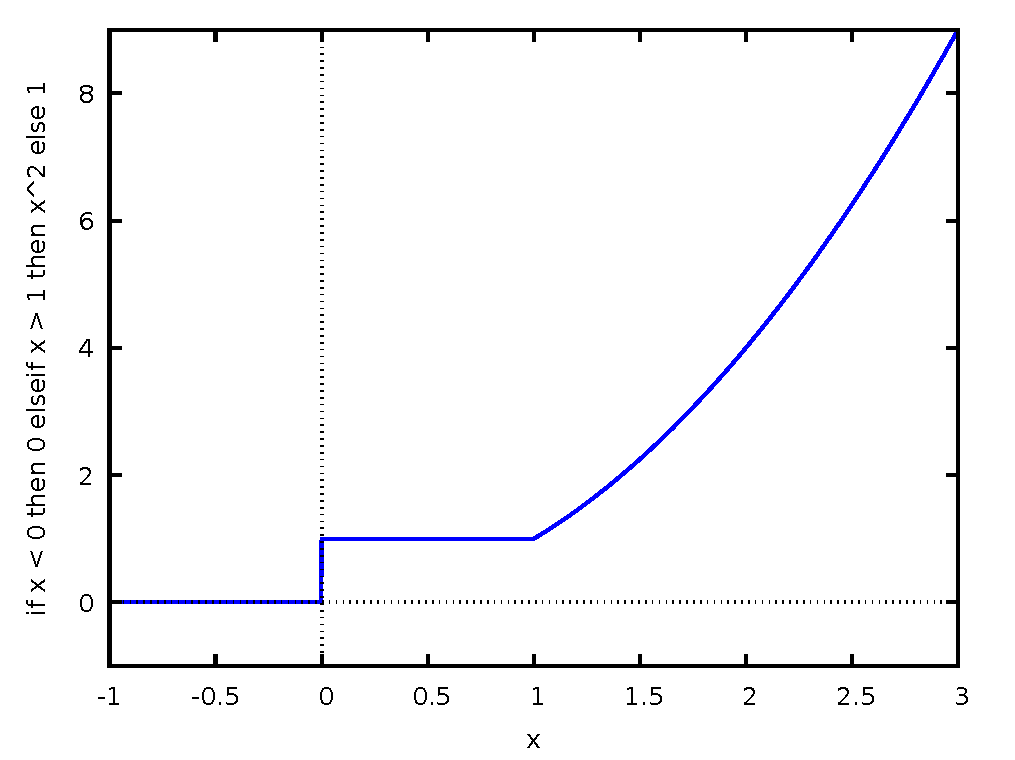
\includegraphics[scale=.5]{plot_G2.pdf}
	\end{center}
\end{maximat}

A continuación veamos varios ejemplos de funciones que usan
condicionales para ser definidas.

La función \maximain{max3} toma tres argumentos y devuelve
el elemento mayor.

\begin{maximai}
	max3(x,y,z):= if (x>=y and x>=z) then x
\end{maximai}\begin{maximal}
	elseif (y>=x and y>=z) then y else z$
\end{maximal}

\begin{maximai}
	max3(-1,5,3);
\end{maximai}
\begin{maximao}
	5
\end{maximao}

La función \maximain{signo} devuelve el signo de un número.

\begin{maximai}
signo(x):=if x>0 then 1 elseif x<0 then -1 else 0$
\end{maximai}

\begin{maximai}
[signo(1),signo(-3),signo(0)];
\end{maximai}
\begin{maximao}
\left[ 1 , -1 , 0 \right] 
\end{maximao}

%\input{bucles}
%!TeX root=main.tex

\section*{Ejercicios}

\begin{enumerate}

	\item Calcule los siguientes números con el número de
dígitos que se indica.
	\begin{enumerate}
		\item $\sqrt{3}$ con $25$ dígitos.
		\item $\pi$ con $30$ dígitos.
		\item $e^2$ con $15$ dígitos.
		\item $\frac{1+\sqrt{5}}{2}$ con $44$ dígitos.
	\end{enumerate}

	\item Escriba en forma decimal los siguientes números con una precisión
de 10 cifras, también calcule los errores absolutos correspondientes.
\begin{equation*}
	\frac{2}{5},\qquad \frac{8}{10}, \qquad \frac{71}{100}.
\end{equation*}

\end{enumerate}


\end{document}
